
\section{Результаты}
\subsection{Гистограммы и графики плотности распределения}
\begin{figure}[H]
    \centering
    \includegraphics[width = 1\linewidth]{hist/normal.png}
    \caption{Нормальное распределение (\ref{eq1})}
    \label{fig1}
\end{figure}

\begin{figure}[H]
    \centering
    \includegraphics[width = 1\linewidth]{hist/cauchy.png}
    \caption{Распределение Коши (\ref{eq2})}
    \label{fig2}
\end{figure}

\begin{figure}[H]
    \centering
    \includegraphics[width = 1\linewidth]{hist/student.png}
    \caption{Распределение Стьюдента (\ref{eq3})}
    \label{fig3}
\end{figure}

\begin{figure}[H]
    \centering
    \includegraphics[width = 1\linewidth]{hist/poisson.png}
    \caption{Распределение Пуассона (\ref{eq4})}
    \label{fig4}
\end{figure}

\begin{figure}[H]
    \centering
    \includegraphics[width = 1\linewidth]{hist/uniform.png}
    \caption{Равномерное распределение (\ref{eq5})}
    \label{fig5}
\end{figure}

\subsection{Характеристики положения}

\begin{table}[H]
    \centering
    \begin{tabular}{ |c|c|c|c|c|c| } 
 \hline
 normal n = 10 & & & & & \\ 
 \hline
  &$\overline{x}\ (\ref{eq6})$ & $med\ x\ (\ref{eq7})$ & $z_{R}\ (\ref{eq8})$ & $z_{Q}\ (\ref{eq10})$ & $z_{tr}\ (\ref{eq11})$\\ 
 \hline
 $E(z)$ & $5,4 \cdot 10^{-3}$ & $-4,4\cdot 10^{-3}$ & $-1,2 \cdot 10^{-2}$ & $7,3 \cdot 10^{-3}$ & $2,4 \cdot 10^{-2}$ \\ 
 \hline
 $D(z)\ (\ref{eq12})$ & $3,2\cdot 10^{-1}$ & $3,7 \cdot 10^{-1}$ & $4,4 \cdot 10^{-1}$ & $3,5 \cdot 10^{-1}$ & $4,1 \cdot 10^{-1}$ \\ 
 \hline\hline
 normal n = 100 & & & & & \\
 \hline
 &$\overline{x}$ & $med\ x$ & $z_{R}$ & $z_{Q}$ & $z_{tr}$\\ 
 \hline
 $E(z)$ & $-1,7 \cdot 10^{-3}$ & $-2,0 \cdot 10^{-3}$ & $-1,1 \cdot 10^{-2}$ & $-1,3 \cdot 10^{-3}$ & $-2,6 \cdot 10^{-3}$ \\ 
 \hline
 $D(z)$ & $9,5 \cdot 10^{-2}$ & $1,2 \cdot 10^{-1}$ & $2,9 \cdot 10^{-1}$ & $1,1 \cdot 10^{-1}$ & $1,4 \cdot 10^{-1}$ \\ 
 \hline\hline
 normal n = 1000 & & & & & \\
 \hline
 &$\overline{x}$ & $med\ x$ & $z_{R}$ & $z_{Q}$ & $z_{tr}$\\ 
 \hline
 $E(z)$ & $-7,0 \cdot 10^{-4}$ & $-1,1 \cdot 10^{-3}$ & $-8,9 \cdot 10^{-3}$ & $0,0 $ & $5,0 \cdot 10^{-4}$ \\ 
 \hline
 $D(z)$ & $3,1 \cdot 10^{-2}$ & $4,0 \cdot 10^{-2}$ & $2,4 \cdot 10^{-1}$ & $3,4 \cdot 10^{-2}$ & $4,4 \cdot 10^{-2}$ \\
 \hline
\end{tabular}
    \caption{Нормальное распределение}
    \label{table:1}
\end{table}


\begin{table}[H]
    \centering
    \begin{tabular}{ |c|c|c|c|c|c| } 
 \hline
 cauchy n = 10 & & & & & \\ 
 \hline
  &$\overline{x}\ (\ref{eq6})$ & $med\ x\ (\ref{eq7})$ & $z_{R}\ (\ref{eq8})$ & $z_{Q}\ (\ref{eq10})$ & $z_{tr}\ (\ref{eq11})$\\ 
 \hline
 $E(z)$ & $3,1 \cdot 10^{-1}$ & $-6,7 \cdot 10^{-3}$ & $ 1,7 $ & $ -4,4 \cdot 10^{-2}$ & $-9,7 \cdot 10^{-1}$ \\ 
 \hline
 $D(z)\ (\ref{eq12})$ & $3,7 \cdot 10^{1}$ & $5,7 \cdot 10^{-1}$ & $1,8 \cdot 10^{2}$ & $9,5 \cdot 10^{-1}$ & $1,6 \cdot 10^{1}$ \\ 
 \hline\hline
 cauchy n = 100 & & & & & \\
 \hline
 &$\overline{x}$ & $med\ x$ & $z_{R}$ & $z_{Q}$ & $z_{tr}$\\ 
 \hline
 $E(z)$ & $1,3$ & $5,3 \cdot 10^{-3}$ & $6,6 \cdot 10^{1}$ & $3,1 \cdot 10^{-3}$ & $3,6$ \\ 
 \hline
 $D(z)$ & $5,2 \cdot 10^{1}$ & $1,6 \cdot 10^{-1}$ & $2,6 \cdot 10^{3}$ & $2,4 \cdot 10^{-1}$ & $8,9 \cdot 10^{1}$ \\ 
 \hline\hline
 cauchy n = 1000 & & & & & \\
 \hline
 &$\overline{x}$ & $med\ x$ & $z_{R}$ & $z_{Q}$ & $z_{tr}$\\ 
 \hline
 $E(z)$ & $-6,4$ & $3,7\cdot 10^{-3}$ & $-3,2 \cdot 10^{3}$ & $6,6 \cdot 10^{-3}$ & $-1,6$ \\ 
 \hline
 $D(z)$ & $1,8 \cdot 10^{2}$ & $5,0 \cdot 10^{-2}$ & $9,2 \cdot 10^{4}$ & $7,0 \cdot 10^{-2}$ & $2,9 \cdot 10^{1}$ \\
 \hline
\end{tabular}
    \caption{Распределение Коши}
    \label{table:2}
\end{table}


\begin{table}[H]
    \centering
    \begin{tabular}{ |c|c|c|c|c|c| } 
 \hline
 student n = 10 & & & & & \\ 
 \hline
  &$\overline{x}\ (\ref{eq6})$ & $med\ x\ (\ref{eq7})$ & $z_{R}\ (\ref{eq8})$ & $z_{Q}\ (\ref{eq10})$ & $z_{tr}\ (\ref{eq11})$\\ 
 \hline
 $E(z)$ & $-5,3 \cdot 10^{-3}$ & $-4,5 \cdot 10^{-3}$ & $-2,6 \cdot 10^{-2}$ & $-3,0 \cdot 10^{-3}$ & $-6,5 \cdot 10^{-3}$ \\ 
 \hline
 $D(z)\ (\ref{eq12})$ & $5,3 \cdot 10^{-1}$ & $4,4 \cdot 10^{-1}$ & $1,4$ & $4,3 \cdot 10^{-1}$ & $6,6 \cdot 10^{-1}$ \\ 
 \hline\hline
 student n = 100 & & & & & \\
 \hline
 &$\overline{x}$ & $med\ x$ & $z_{R}$ & $z_{Q}$ & $z_{tr}$\\ 
 \hline
 $E(z)$ & $1,0 \cdot 10^{-2}$ & $4,2 \cdot 10^{-3}$ & $1,1 \cdot 10^{-1}$ & $2,5 \cdot 10^{-3}$ & $6,2 \cdot 10^{-3}$ \\ 
 \hline
 $D(z)$ & $1,7 \cdot 10^{-1}$ & $1,4 \cdot 10^{-1}$ & $2,7$ & $1,4 \cdot 10^{-1}$ & $2,4 \cdot 10^{-1}$ \\ 
 \hline\hline
 student n = 1000 & & & & & \\
 \hline
 &$\overline{x}$ & $med\ x$ & $z_{R}$ & $z_{Q}$ & $z_{tr}$\\ 
 \hline
 $E(z)$ & $3,1 \cdot 10^{-3}$ & $-2,0 \cdot 10^{-4}$ & $1,7 \cdot 10^{-1}$ & $1,7 \cdot 10^{-3}$ & $2,1 \cdot 10^{-3}$ \\ 
 \hline
 $D(z)$ & $5,5 \cdot 10^{-2}$ & $4,4 \cdot 10^{-2}$ & $6,0$ & $4,4 \cdot 10^{-2}$ & $7,7 \cdot 10^{-2}$ \\
 \hline
\end{tabular}
    \caption{Распределение Стьюдента}
    \label{table:3}
\end{table}


\begin{table}[H]
    \centering
    \begin{tabular}{ |c|c|c|c|c|c| } 
 \hline
 poisson n = 10 & & & & & \\ 
 \hline
  &$\overline{x}\ (\ref{eq6})$ & $med\ x\ (\ref{eq7})$ & $z_{R}\ (\ref{eq8})$ & $z_{Q}\ (\ref{eq10})$ & $z_{tr}\ (\ref{eq11})$\\ 
 \hline
 $E(z)$ & $1,0 \cdot 10^{1}$ & $9.9$ & $1,0 \cdot 10^{1}$ & $9.9$ & $1,0 \cdot 10^{1}$ \\ 
 \hline
 $D(z)\ (\ref{eq12})$ & $1,0$ & $1,2$ & $1,4$ & $1,1$ & $1,3$ \\ 
 \hline\hline
 poisson n = 100 & & & & & \\
 \hline
 &$\overline{x}$ & $med\ x$ & $z_{R}$ & $z_{Q}$ & $z_{tr}$\\ 
 \hline
 $E(z)$ & $1,0 \cdot 10^{1}$ & $9.9$ & $1,1 \cdot 10^{1}$ & $9.9$ & $1,0 \cdot 10^{1}$ \\ 
 \hline
 $D(z)$ & $3,0 \cdot 10^{-1}$ & $4,1 \cdot 10^{-1}$ & $9,6 \cdot 10^{-1}$ & $3,8 \cdot 10^{-1}$ & $4,3 \cdot 10^{-1}$ \\ 
 \hline\hline
 poisson n = 1000 & & & & & \\
 \hline
 &$\overline{x}$ & $med\ x$ & $z_{R}$ & $z_{Q}$ & $z_{tr}$\\ 
 \hline
 $E(z)$ & $1,0 \cdot 10^{1}$ & $1,0 \cdot 10^{1}$ & $1,2 \cdot 10^{1}$ & $1,0 \cdot 10^{1}$ & $1,0 \cdot 10^{1}$ \\ 
 \hline
 $D(z)$ & $9,6 \cdot 10^{-2}$ & $3,5 \cdot 10^{-2}$ & $8,1 \cdot 10^{-1}$ & $3,6 \cdot 10^{-2}$ & $1,4 \cdot 10^{-1}$ \\
 \hline
\end{tabular}
    \caption{Распределение Пуассона}
    \label{table:4}
\end{table}


\begin{table}[H]
    \centering
    \begin{tabular}{ |c|c|c|c|c|c| }
 \hline
 uniform n = 10 & & & & & \\ 
 \hline
  &$\overline{x}\ (\ref{eq6})$ & $med\ x\ (\ref{eq7})$ & $z_{R}\ (\ref{eq8})$ & $z_{Q}\ (\ref{eq10})$ & $z_{tr}\ (\ref{eq11})$\\ 
 \hline
 $E(z)$ & $1,8 \cdot 10^{-2}$ & $8,9 \cdot 10^{-3}$ & $1,5 \cdot 10^{-2}$ & $2,2 \cdot 10^{-2}$ & $5,9 \cdot 10^{-3}$ \\ 
 \hline
 $D(z)\ (\ref{eq12})$ & $3,3 \cdot 10^{-1}$ & $4,9 \cdot 10^{-1}$ & $2,1 \cdot 10^{-1}$ & $3,9 \cdot 10^{-1}$ & $4,2 \cdot 10^{-1}$ \\ 
 \hline\hline
 uniform n = 100 & & & & & \\
 \hline
 &$\overline{x}$ & $med\ x$ & $z_{R}$ & $z_{Q}$ & $z_{tr}$\\ 
 \hline
 $E(z)$ & $-2,2 \cdot 10^{-3}$ & $-4,5 \cdot 10^{-3}$ & $-8,0 \cdot 10^{-4}$ & $-3,0 \cdot 10^{-4}$ & $4,0 \cdot 10^{-4}$ \\ 
 \hline
 $D(z)$ & $1,0 \cdot 10^{-1}$ & $1,7 \cdot 10^{-1}$ & $2,4 \cdot 10^{-2}$ & $1,2 \cdot 10^{-1}$ & $1,3 \cdot 10^{-1}$ \\ 
 \hline\hline
 uniform n = 1000 & & & & & \\
 \hline
 &$\overline{x}$ & $med\ x$ & $z_{R}$ & $z_{Q}$ & $z_{tr}$\\ 
 \hline
 $E(z)$ & $-6,0 \cdot 10^{-4}$ & $5,0 \cdot 10^{-4}$ & $0,0$ & $-7,0 \cdot 10^{-4}$ & $1,0 \cdot 10^{-4}$ \\ 
 \hline
 $D(z)$ & $3,1 \cdot 10^{-2}$  &$5,4 \cdot 10^{-2}$ & $2,4 \cdot 10^{-3}$ &  $3,9 \cdot 10^{-2}$ & $4,4 \cdot 10^{-2}$ \\
 \hline
\end{tabular}
    \caption{Равномерное распределение}
    \label{table:5}
\end{table}

\subsection{Бокс-плот Тьюки}

\begin{figure}[H]
    \centering
    \includegraphics[width = 1\linewidth]{tukey/normal.png}
    \caption{Бокс-плот Тьюки для нормального распределения (\ref{eq1})}
    \label{fig6}
\end{figure}

\begin{figure}[H]
    \centering
    \includegraphics[width = 1\linewidth]{tukey/cauchy.png}
    \caption{Бокс-плот Тьюки для распределения Коши (\ref{eq2})}
    \label{fig7}
\end{figure}

\begin{figure}[H]
    \centering
    \includegraphics[width = 1\linewidth]{tukey/student.png}
    \caption{Бокс-плот Тьюки для распределения Стьюдента (\ref{eq3})}
    \label{fig8}
\end{figure}

\begin{figure}[H]
    \centering
    \includegraphics[width = 1\linewidth]{tukey/poisson.png}
    \caption{Бокс-плот Тьюки для распределения Пуассона (\ref{eq4})}
    \label{fig9}
\end{figure}

\begin{figure}[H]
    \centering
    \includegraphics[width = 1\linewidth]{tukey/uniform.png}
    \caption{Бокс-плот Тьюки для равномерного распределения (\ref{eq5})}
    \label{fig10}
\end{figure}

\subsection{Доверительные интервалы для параметров распределений}

\begin{table}[H]
\centering
\begin{tabular}{ |c|c|c| } 
 \hline
 $n = 20$ & $m$(\ref{eq16}) & $\sigma$ (\ref{eq17})\\ 
 \hline
  & -0,46 < $m$ < 0,37 & 0,67 < $\sigma$ < 1,29\\ 
  \hline
  $n = 100$ & $m$ & $\sigma$ \\
  \hline
  & -0,25 < $m$ < 0,11 & 0,80 < $\sigma$ < 1,10\\ 
 \hline
\end{tabular}
\caption{Доверительные интервалы для параметров нормального распределения}
    \label{table:6}
\end{table}

\begin{table}[H]
\centering
\begin{tabular}{ |c|c|c| } 
 \hline
 $n = 20$ & $m$(\ref{eq18}) & $\sigma$ (\ref{eq19})\\ 
 \hline
  & -1,32 < $m$ < 1,05 & 1,74 < $\sigma$ < 3,68\\ 
  \hline
  $n = 100$ & $m$ & $\sigma$ \\
  \hline
  & -1,10 < $m$ < 1,13 & 3,31 < $\sigma$ < 8,10 \\ 
 \hline
\end{tabular}
\caption{Доверительные интервалы для параметров распределения Коши}
    \label{table:7}
\end{table}

\begin{table}[H]
\centering
\begin{tabular}{ |c|c|c| } 
 \hline
 $n = 20$ & $m$(\ref{eq18}) & $\sigma$ (\ref{eq19})\\ 
 \hline
  & -0,85 < $m$ < 0,73 & 0,98 < $\sigma$ < 2,62\\ 
  \hline
  $n = 100$ & $m$ & $\sigma$ \\
  \hline
  & 0,0083 < $m$ < 0,53 & 1,10 < $\sigma$ < 1,58 \\ 
 \hline
\end{tabular}
\caption{Доверительные интервалы для параметров распределения Стьюдента}
    \label{table:8}
\end{table}

\begin{table}[H]
\centering
\begin{tabular}{ |c|c|c| } 
 \hline
 $n = 20$ & $m$(\ref{eq18}) & $\sigma$ (\ref{eq19})\\ 
 \hline
  & 8,36 < $m$ < 10,74 & 1,62 < $\sigma$ < 3,78\\ 
  \hline
  $n = 100$ & $m$ & $\sigma$ \\
  \hline
  & 9,30 < $m$ < 10,54 & 2,75 < $\sigma$ < 3,54 \\ 
 \hline
\end{tabular}
\caption{Доверительные интервалы для параметров распределения Пуассона}
    \label{table:9}
\end{table}

\begin{table}[H]
\centering
\begin{tabular}{ |c|c|c| } 
 \hline
 $n = 20$ & $m$(\ref{eq18}) & $\sigma$ (\ref{eq19})\\ 
 \hline
  & -0,47 < $m$ < 0,31 & 0,73 < $\sigma$ < 1,05\\ 
  \hline
  $n = 100$ & $m$ & $\sigma$ \\
  \hline
  & -0,19 < $m$ < 0,19 & 0,89 < $\sigma$ < 1,07 \\ 
 \hline
\end{tabular}
\caption{Доверительные интервалы для параметров равномерного распределения}
    \label{table:10}
\end{table}

\begin{figure}[H]
    \centering
    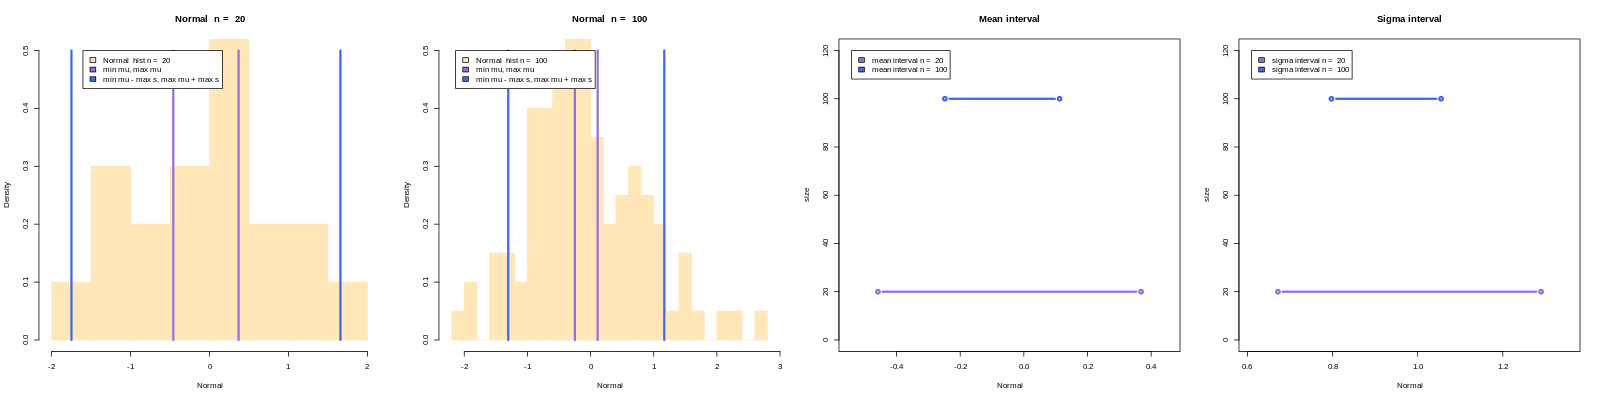
\includegraphics[width = 1\linewidth]{images/ranges/normal.png}
    \caption{Гистограммы и оценки для параметров нормального распределения}
    \label{fig11}
\end{figure}

\begin{figure}[H]
    \centering
    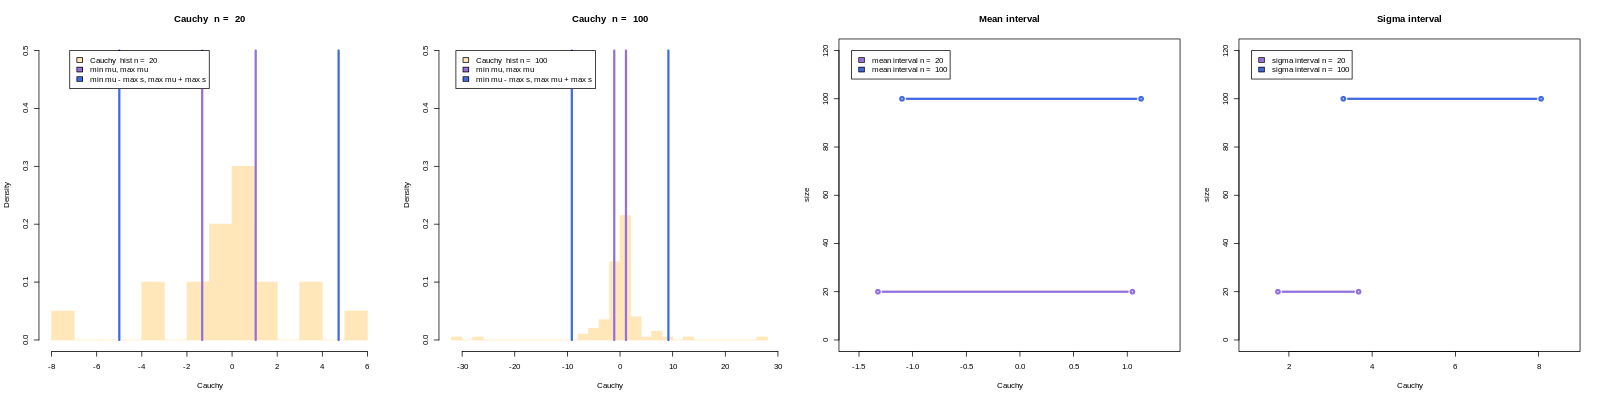
\includegraphics[width = 1\linewidth]{images/ranges/cauchy.png}
    \caption{Гистограммы и оценки для параметров распределения Коши}
    \label{fig12}
\end{figure}

\begin{figure}[H]
    \centering
    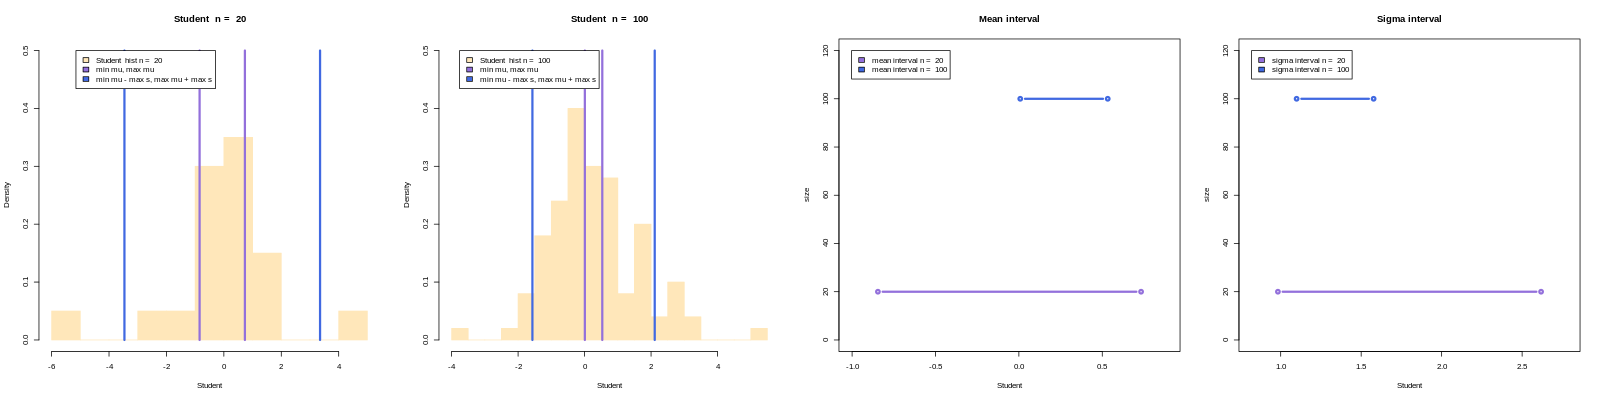
\includegraphics[width = 1\linewidth]{images/ranges/student.png}
    \caption{Гистограммы и оценки для параметров распределения Сьюдента}
    \label{fig13}
\end{figure}

\begin{figure}[H]
    \centering
    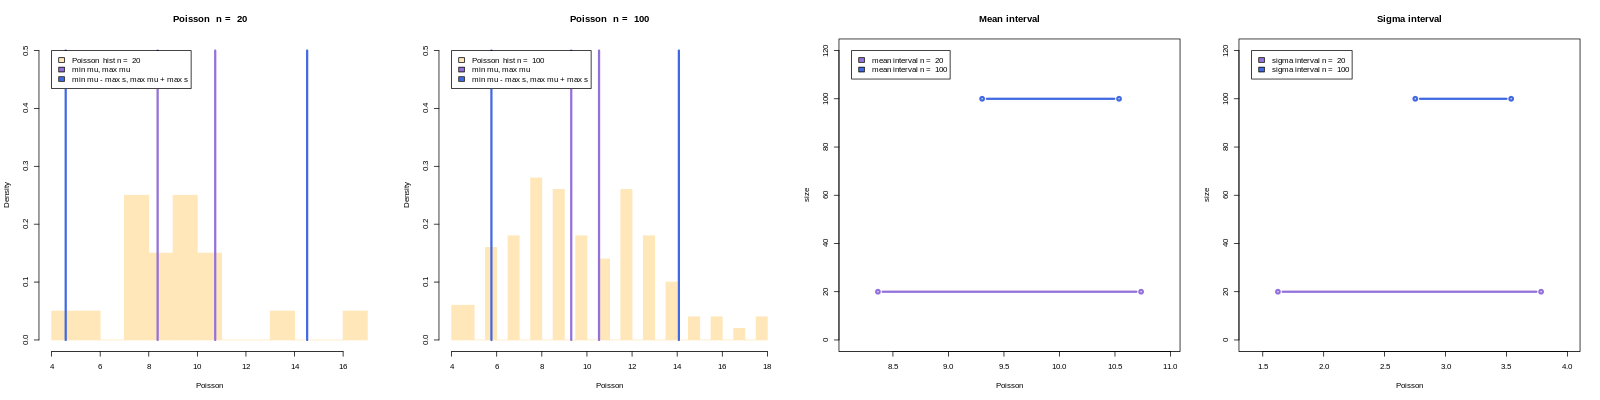
\includegraphics[width = 1\linewidth]{images/ranges/poisson.png}
    \caption{Гистограммы и оценки для параметров распределения Пуассона}
    \label{fig14}
\end{figure}

\begin{figure}[H]
    \centering
    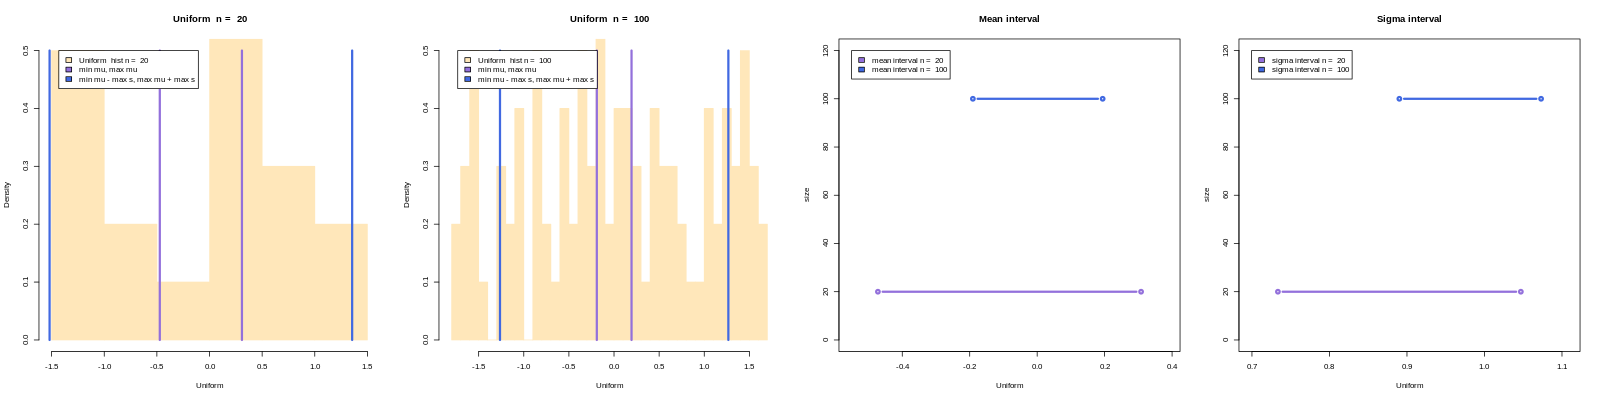
\includegraphics[width = 1\linewidth]{images/ranges/uniform.png}
    \caption{Гистограммы и оценки для параметров равномерного распределения}
    \label{fig15}
\end{figure}
